\chapter{Testing}
\section{Stochastic model}
\subsection{Birth rate} \label{sec:model:birthrate}
In order to evaluate the birth rate at a given depth, the following equation models a production process which saturates (see \autoref{sec:math-model}):
\begin{equation}
  f(z,t) = \lambda \frac{I(z,t)}{H + I(z,t)}
\end{equation}
where
\[ I(z,t) = e^{-k_{bg}z-k_{ss}\int_0^z n(z,t)} \]
Converting this equation to a discrete context, at a given time, for a given particle $i$
\[ I(i) = e^{-k_{bg}z_i - k_{ss}\sum_{\{\hat{j}\}}1} \]
where $\hat{j}$ represents the indexes of particles which are at a shallower depth than the one labelled with $i$.
However, this exact method of summing the particles is computationally expensive, since one has to nest two loops over the particles: the inner one increments the value of the sum with the condition above, while the outer one assigns this value to the $i$th cell, resulting in a $\mathcal{O}(N^2)$ operation. A much faster way to approach this is to fill a histogram with the cells, then sum incrementally over the bins in order to get the value of the sum on a discrete set of points; now it is possible to assign the birth rates either choosing the upper (or lower) value on the grid, or interpolating with the following linear espression:
\[ f(x) \simeq (x_2-x)f(x_1)+(x-x_1)f(x_2) \]
Some comparisons are shown in \autoref{fig:compare_integral}, from a simulation run with 1000 cells: an error has to be expected due to the approximation, but for the most part of the points it is below 10\%; even better when considering the estimate of the birth rate, where the errors are well below 1\%. Considering that the birth rate is actually the interesting quantity, the approximation is acceptable and it has been used instead of the exact method in order to make the code faster.

\begin{figure}
 \begin{subfigure}[b]{0.45\textwidth}
    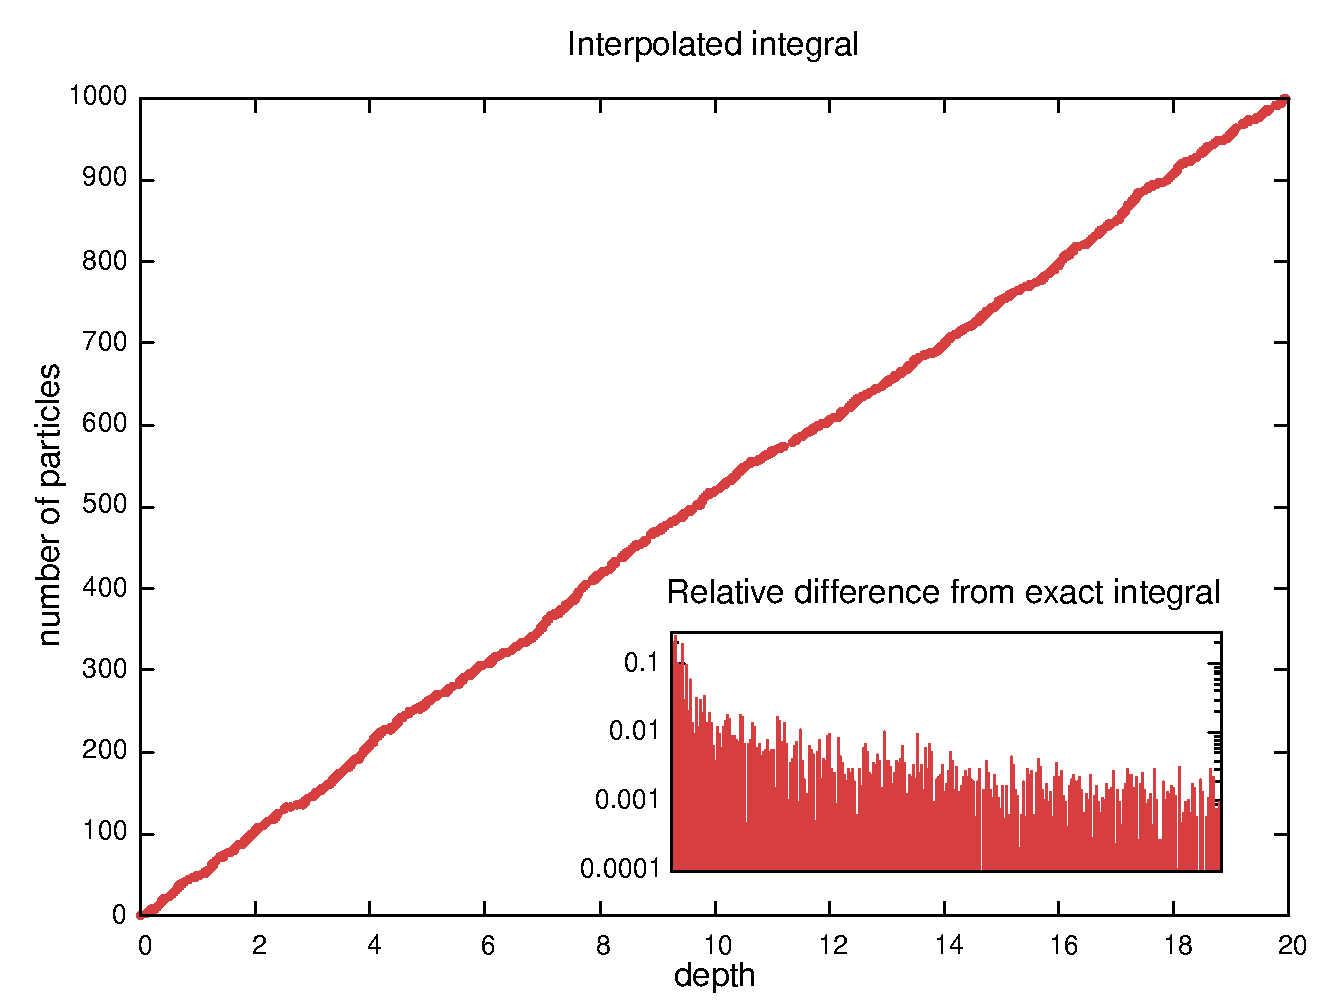
\includegraphics[width=\textwidth]{data/1D_model/test_integral/interpolated_integral}
    \caption{}
    \label{fig:interpolated_integral}
  \end{subfigure}
  %add desired spacing between images, e. g. ~, \quad, \qquad, \hfill etc. 
  %(or a blank line to force the subfigure onto a new line)
  \begin{subfigure}[b]{0.45\textwidth}
    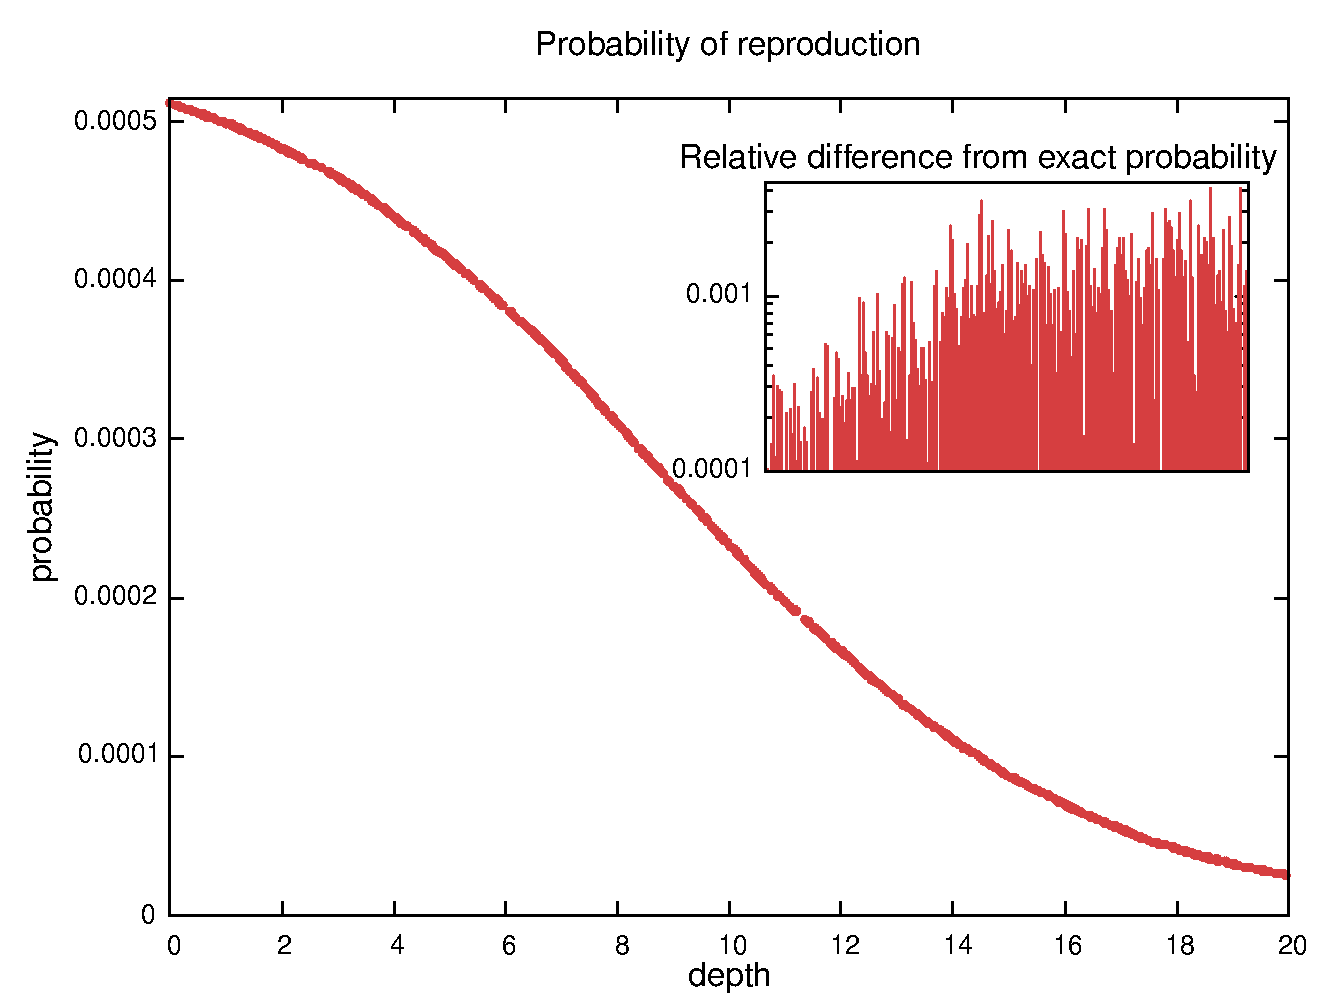
\includegraphics[width=\textwidth]{data/1D_model/test_integral/interpolated_preproduction}
    \caption{}
    \label{fig:interpolated_preproduction}
  \end{subfigure}
  \caption{Comparison between the exact and interpolated methods described in \autoref{sec:model:birthrate}. In \autoref{fig:interpolated_integral} the interpolated integral is shown for each particle in the simulation, with an inset concerning the relative deviations from the exact integral; in \autoref{fig:interpolated_preproduction}, the same is made for the reproduction rate.}
  \label{fig:compare_integral}
\end{figure}



\subsection{No-flux conditions} \label{sec:no-flux-test}

In this numerical model, the following implementation for the boundary conditions has been used, where \(x' = v \mathrm{d}t + \sqrt{2D\cdot \mathrm{d}t}\zeta\) as in \autoref{eq:eul-difadv}:
\begin{equation}
x_i^{n+1} = \begin{cases}
    x' &\mathrm{if}\; x' \in [x_{min},x_{max}] \\
    2x_{min} - x' &\mathrm{if}\; x' < x_{min} \\
    2x_{max} - x' &\mathrm{if}\; x' > x_{max} 
\end{cases}
\end{equation}

\paragraph{Validation}
In order to validate the model, some testing is performed about no-flux conditions.
The one-dimensional diffusion-advection equation
\begin{equation} \label{eq:n-difadv}
  \partial_t n(x,t) = -v\partial_x n(x,t) +D\partial^2_x n(x,t) 
\end{equation}
is considered: $n$ represents a density of particles, diffused with a coefficient $D$ and advected towards biggest values of $x$ (for positive values of $v$). This equation relates to the 1-dimensional phytoplankton model by imposing both the production and loss factors to 0. An analytic solution can be derived for closed boundaries: defining the current \( J := vn - D\partial_x n \), 
the no-flux conditions at a point $\bar{x}$ can be written as (\autocite{Huisman2002HowPersist})
\begin{equation} \label{eq:noflux}
J(\bar{x}) = 0
\end{equation}
and \autoref{eq:n-difadv} becomes
\[ \partial_t n + \partial_x J = 0 \]
The following steady-state condition holds:
\[ \partial_x J = 0 \]
Defining the auxiliary variable \( \xi=\xi\partial_xn \) a solution is 
\[ \xi(x) = \xi_0 e^{\frac{v(x-x_0)}{D}} \]
where $x_0$ is the lowest value of $x$; this gives
\[ n(x) = \xi_0 \frac{D}{v} e^{\frac{v(x-x_0)}{D}} + n_0 \;\;. \]
and 
\[ J(x) = v n_0 = const \]
Imposing no-flux conditions means 
\[ J(x_0) = vn_0 = 0 \;\; \Rightarrow \;\; n_0 = 0\]
so the general solution with no-flux boundaries is
\begin{equation} \label{eq:rho-noflux-da}
  n(x) = \alpha \frac{D}{v} e^{\frac{v(x-x_0)}{D}} \;\;.
\end{equation}
where $\alpha$ is a constant depending on the initial conditions.
A formula for this constant can be obtained evaluating the number of particles
\[ N(x) = \int_{x_0}^{x} n(x) \mathrm{d}x = \alpha \frac{D}{v} \left( e^{\frac{v(x-x_0)}{D}} - 1 \right) \]
which gives
\begin{equation} \label{eq:rho-noflux-const}
  \alpha =\frac{N(x)}{\left(\frac{D}{v}\right)^2\left( e^{\frac{v(x-x_0)}{D}} - 1 \right)}
\end{equation}

% The Eulerian integration is performed in an interval \( [0,1] \), where $10^5$ particles are uniformly distributed at time zero (since we are looking for a stationary solution, this detail is not influent). The parameters used in the simulation are listed in \autoref{tab:eul-par}.
This analytic result serves as a test distribution which has to be matched by the model developed. 
\autoref{eq:rho-noflux-const} with the parameters in \autoref{tab:eul-par}, used for the simulation, becomes 
\[ \alpha = \frac{1}{(e-1)n_{bin}} \]
where $n_{bin}$ is the number of bins of the histogram, introduced because of the normalization. \\
As can be seen in \autoref{img:bound-refl-fit}, the fit is good, thus confirming that the chosen implementation of no-flux conditions is consistent.

\begin{table} 
  \begin{center}
    \begin{tabular}{ c | c | c | c} 
      \hline
      D               & v             & $z_0$    & $z_{max}$ \\ \hline
      $0.01m^2h^{-1}$ & $0.01mh^{-1}$ & $0m$     & $1m$        \\
      \hline
    \end{tabular}
  \end{center}
  \caption{Parameters used for the simulation of \autoref{eq:eul-difadv}. }
  \label{tab:eul-par}
\end{table}

\begin{figure}[!htb]
  \centering
  \begin{subfigure}[b]{0.4\textwidth}
    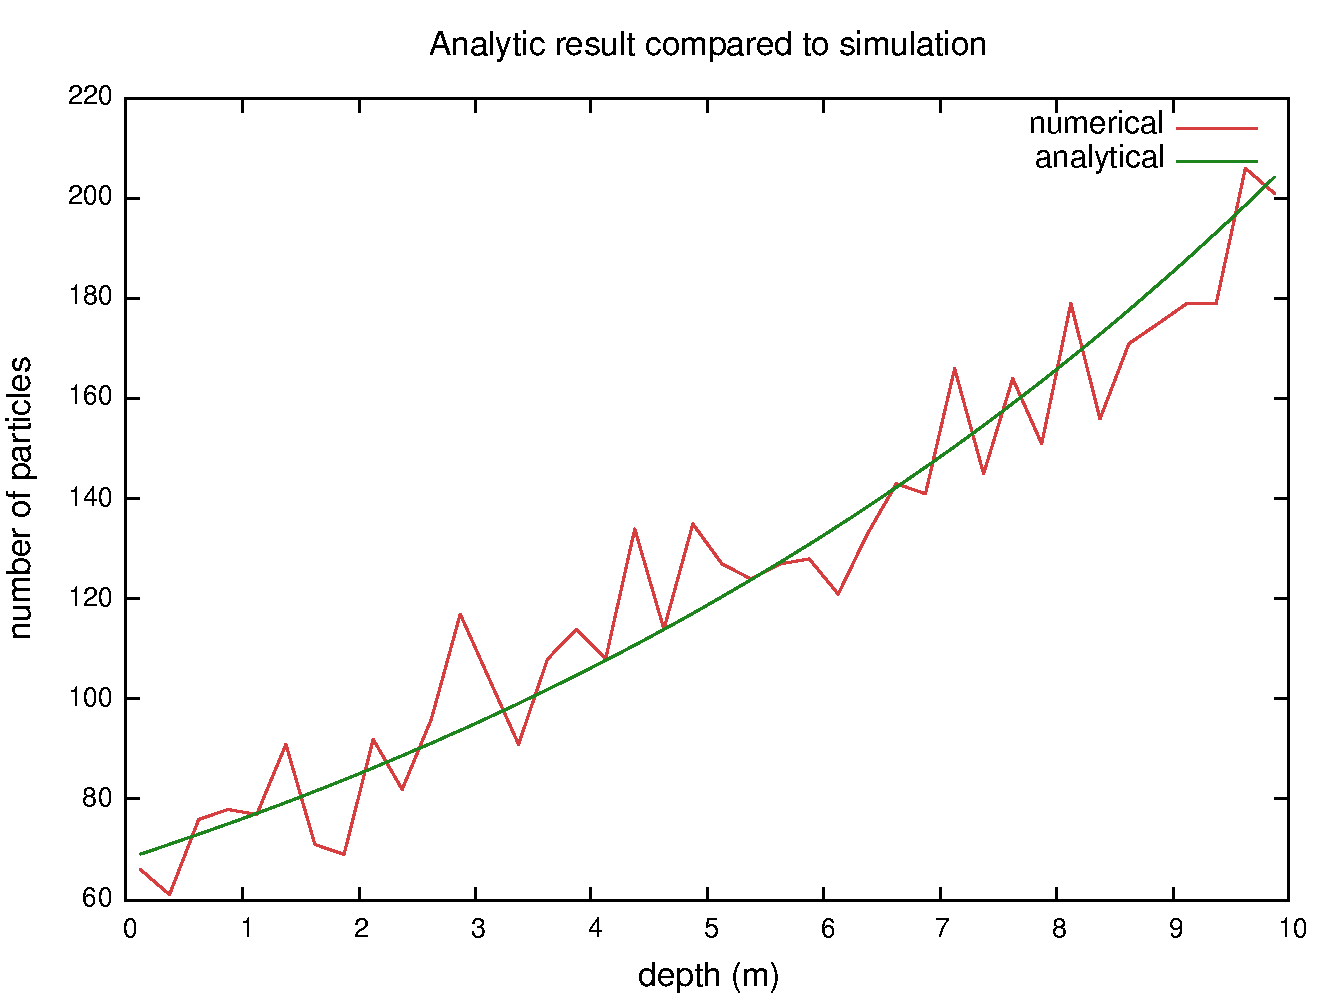
\includegraphics[width=1\textwidth]{data/1D_model/reflective_bottom/noflux_conditions/cfr_stoc_refl}
    \caption{}
    \label{img:bound-refl-fit}
  \end{subfigure}
  \begin{subfigure}[b]{0.4\textwidth}
    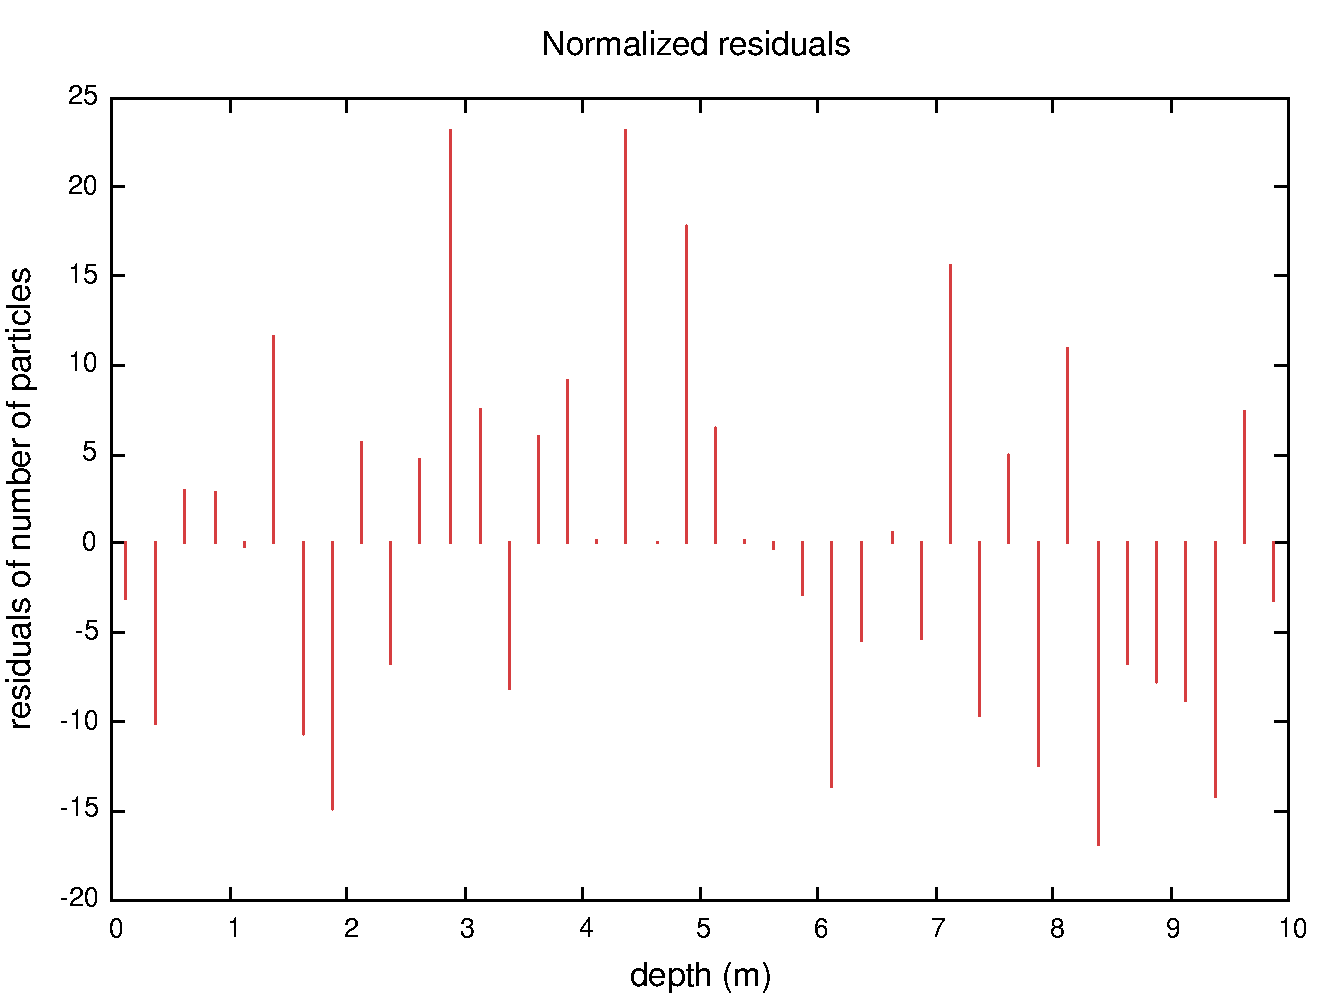
\includegraphics[width=1\textwidth]{data/1D_model/reflective_bottom/noflux_conditions/cfr_stoc_refl_residuals}
    \caption{}
    \label{img:bound-refl-fit-residuals}
  \end{subfigure}
  \caption{In \autoref{img:bound-refl-fit} the fit is shown of the distribution of particles averaged near equilibrium, according to \autoref{eq:eul-difadv}, with parameters in \autoref{tab:eul-par}. 
  In \autoref{img:bound-refl-fit-residuals} the residuals of the actual distribution with respect to the analytic one are plotted.
  Simulation run with $2500$ particles.}
\end{figure}

\section{Lagrangian model}
In order to check the consistence of the numerical model with expected results, some tests are performed.

%\subsection{Sinking velocity}
%The Lagrangian code is modified in order to nullify the effects of advective flow and reactions of the cells. Since $dt=5\cdot10^{-3}$ and $v=1$, after $1000$ iterations the particles are expected to have travelled $5$.


\subsection{Light intensity}
%Run with (make copies of files):
%\begin{itemize}
%    \item initial random particle distribution
%    \item position does not evolve (use no\_advection)
%    \item $\lambda=0$, $\mu=0$
%    \item in popul.f90 write $(x_{particle},intens)$
%    \item look at "denso.xxx"
%\end{itemize}
%Profile should be exponential (integral over depth is linear) and in 0 should be =1.
In particular, since the distribution here is uniform, given $N$ total particles it will result \( \int_0^z n(r) \mathrm{d}r \sim \int_0^z \frac{N}{L_z} \mathrm{d}r = z\frac{N}{L_z} \) so that, following \autoref{eq:generic_light},
\begin{equation} \label{eq:light_func}
    \frac{I(z)}{I_0} \sim e^{-z(k_{bg}+k_{ss}\frac{N}{L_z})} 
\end{equation}
The numerical results are compared with these analytical results in \autoref{fig:3d:light_profile}; the residuals are shown in \autoref{fig:3d:light_residuals} and, normalized, in \autoref{fig:3d:light_residuals_relative}; the light as perceived by the particles is plotted in \autoref{fig:3d:light_seen_particles}.

\begin{figure} 
  \centering
  \begin{subfigure}[b]{\textwidth}
    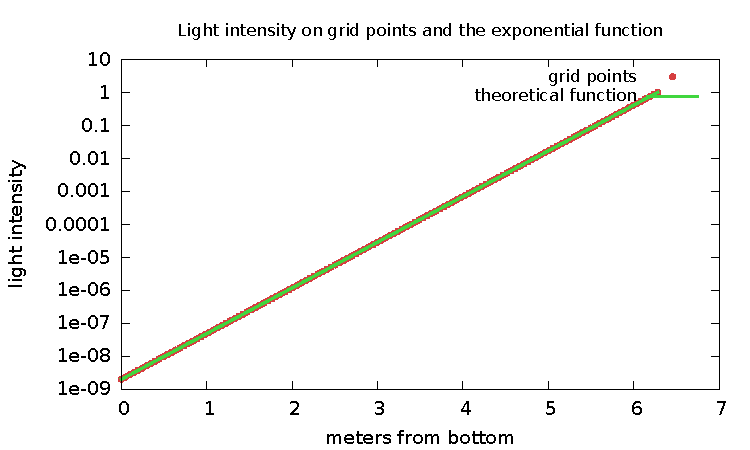
\includegraphics[width=\textwidth]{data/3D_model/light_profile}
    \caption{}
    \label{fig:3d:light_profile}
  \end{subfigure}
  \begin{subfigure}[b]{\textwidth}
    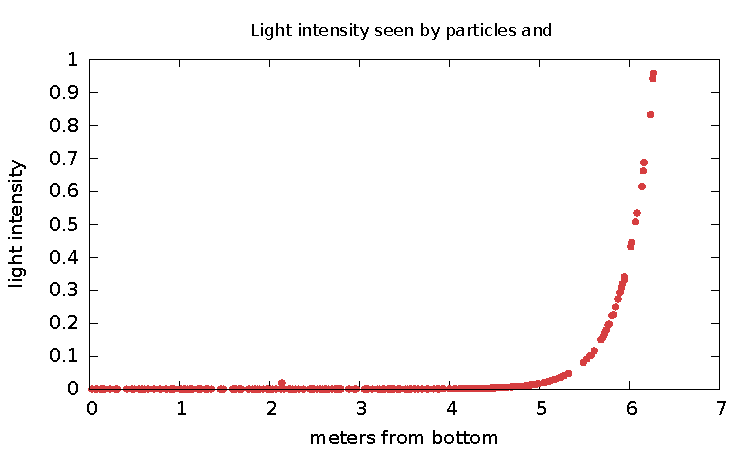
\includegraphics[width=\textwidth]{data/3D_model/light_seen_particle}
    \caption{}
    \label{fig:3d:light_seen_particles}
  \end{subfigure}
    \caption{In \autoref{fig:3d:light_profile} the light intensity set at grid-points is plotted against the theoretical function \autoref{eq:light_func} (see \autoref{sec:ref_crit_turb}); in \autoref{fig:3d:light_seen_particles} the light intensity as seen by each particle is plotted in function of their position.}
    \label{fig:3d_light_A}
\end{figure}
\begin{figure} 
  \centering
  \begin{subfigure}[b]{\textwidth}
    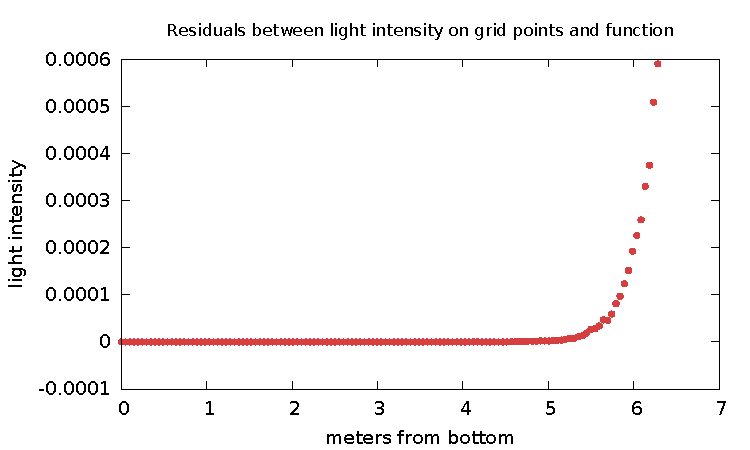
\includegraphics[width=\textwidth]{data/3D_model/light_residuals}
    \caption{}
    \label{fig:3d:light_residuals}
  \end{subfigure}
  
  \begin{subfigure}[b]{\textwidth}
    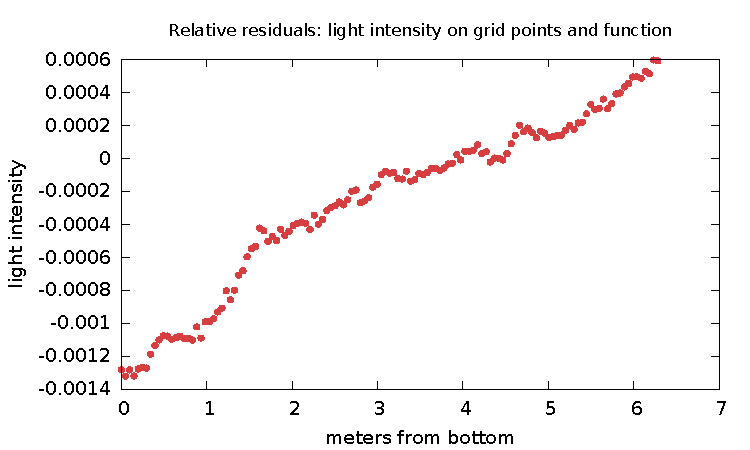
\includegraphics[width=\textwidth]{data/3D_model/light_residuals_relative}
    \caption{}
    \label{fig:3d:light_residuals_relative}
  \end{subfigure}
  \caption{The residuals are shown of light intensity with respect to the theoretical function \autoref{eq:light_func} (see \autoref{fig:3d:light_profile}): in \autoref{fig:3d:light_residuals} the simple difference is considered, while in \autoref{fig:3d:light_residuals_relative} a normalization on by the intensity value has been made.}
    \label{fig:3d_light_B}
\end{figure}


\subsection{Growth reaction}
Modifying the code to eliminate transport both by advective flow and sinking velocity, an exponential growth should be seen if $k_as$ (the auto-shading parameter) is set to zero. The modeling equation is (see \autoref{eq:n-difadv})
\[ \partial_t n(t,z) = \left(\frac{\lambda}{1+\frac{h}{I_0}e^{k_{bg}z}} -\mu\right)n(t,z) = f(z)n(t,z)\]
so the resulting numerical density at a depth $z$ is
\[ n(t,z) = n(0,z)e^{f(z)t} . \]


